\chapter{Special Relativity: Composition of Boosts, Proper Interval, and Four-Vectors}

We begin exactly where the lecture begins: back on the one-dimensional railroad track, with one observer at the station and another in the train. These companion notes follow Leonard Susskind's lecture closely, with transcript and frame curation prepared by LazyingArt LLC and Video2Book. The first task is to recover the geometry already hidden in the Lorentz transformation itself; the second is to compose two boosts and discover the relativistic rule for adding velocities; and the third is to step back from the algebra and reorganize the whole discussion around the invariant interval and the language of four-vectors.

\section{Two Frames, One Axis, and the Choice \(c=1\)}

The lecture opens with a reminder that we are working, for the moment, in a deliberately simplified setting. All relative motion is taken to lie along a single axis, and we imagine a long railroad track with stationary observers at the station and moving observers riding in the train. The basic hypothesis is Einstein's: every inertial observer assigns the same value to the speed of light.

It is convenient to choose units so that this common value is \(1\). In such relativistic units, velocities are dimensionless and the formulas become transparent. When we want to return to conventional units, we put factors of \(c\) back in by requiring dimensional consistency.

An event is a point of spacetime. One may picture it as a flash bulb going off somewhere, perhaps inside the train. The stationary observer assigns coordinates \((x,t)\) to that event, while the observer in the train assigns \((x',t')\). The Lorentz transformations relating the two are
\begin{align}
x' &= \frac{x-vt}{\sqrt{1-v^2}}, &
t' &= \frac{t-vx}{\sqrt{1-v^2}}.
\end{align}
They may also be inverted:
\begin{align}
x &= \frac{x'+vt'}{\sqrt{1-v^2}}, &
t &= \frac{t'+vx'}{\sqrt{1-v^2}}.
\end{align}
For a boost along the \(x\)-axis, the transverse directions are unchanged,
\begin{equation}
y'=y,
\qquad
z'=z.
\end{equation}

The reciprocal character of the transformation is important. Going back from primed to unprimed coordinates does not require a new idea; it requires only the same structure with the sign of the relative velocity reversed. Already at this stage, the lecture insists that these formulas are not abstract algebra. They describe how rods and clocks at rest in one frame correlate with rods and clocks at rest in another.

\section{Reading Motion Off the Lorentz Transformation}

One of the most useful moves in the lecture is also one of the simplest. Instead of staring at the whole transformation, we ask what it says about the origin of the primed coordinates. The primed observer is at rest in his own frame, so his position is characterized by
\begin{equation}
x'=0.
\end{equation}
Setting the numerator of the transformation to zero gives
\begin{equation}
x-vt=0,
\qquad\text{so}\qquad
x=vt.
\end{equation}
The denominator plays no role in locating the line \(x'=0\). What matters is that the worldline of the primed origin, viewed in unprimed coordinates, is the straight line \(x=vt\). In other words, the Lorentz transformation itself tells us the relative velocity.

\begin{figure}[t]
\centering

\includegraphics[width=0.78\textwidth]{lecture_02_figure_02.png}
\caption{Board sketch used to identify the primed origin inside the train. The crucial visible label is \(x'=0\), read against the unprimed coordinates \(x,t\).}
\end{figure}

The board sketch is schematic rather than analytic. The train is drawn as a box, the passenger sits inside it, the station observer sits below, and a dashed projection ties an event in the train to a location on the stationary line. The point of the figure is not metric precision. The point is to see that the primed origin occupies a definite place in the moving carriage, and that this place sweeps out the line \(x=vt\) in the unprimed description.

\begin{figure}[t]
\centering
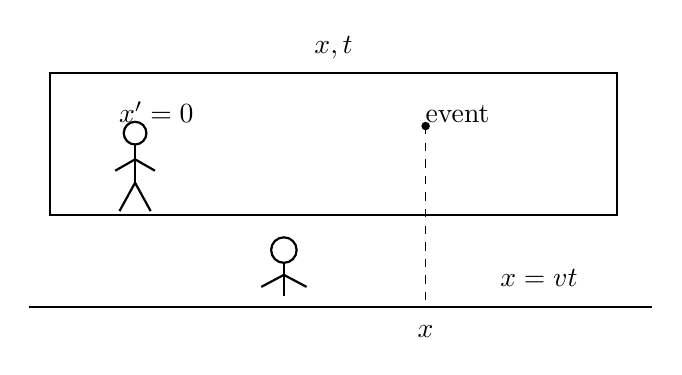
\begin{tikzpicture}[scale=0.9]
\draw[thick] (0,2.2) rectangle (8,4.2);
\draw (4,4.55) node {$x,t$};

\draw[thick] (-0.3,0.9) -- (8.5,0.9);

\draw[thick] (1.2,3.35) circle (0.16);
\draw[thick] (1.2,3.18) -- (1.2,2.65);
\draw[thick] (1.2,2.98) -- (0.92,2.82);
\draw[thick] (1.2,2.98) -- (1.48,2.82);
\draw[thick] (1.2,2.65) -- (0.98,2.25);
\draw[thick] (1.2,2.65) -- (1.42,2.25);
\draw (1.5,3.65) node {$x'=0$};

\fill (5.3,3.45) circle (0.06);
\draw[dashed] (5.3,3.45) -- (5.3,0.9);
\draw (5.75,3.62) node {event};

\draw[thick] (3.3,1.7) circle (0.18);
\draw[thick] (3.3,1.52) -- (3.3,1.05);
\draw[thick] (3.3,1.35) -- (2.98,1.18);
\draw[thick] (3.3,1.35) -- (3.62,1.18);

\draw (5.3,0.55) node {$x$};
\draw (6.9,1.3) node {$x=vt$};
\end{tikzpicture}
\caption{Cleaned schematic of the same construction. The lecture's claim is only that the line \(x'=0\) in the train frame is the line \(x=vt\) in the station frame.}
\end{figure}

\section{A Third Observer and the Composition of Boosts}

Now comes the main exercise of the lecture. We introduce a third observer: a child riding a kiddie car inside the train. The station frame remains \((x,t)\), the train frame remains \((x',t')\), and the kiddie-car frame is denoted by \((x'',t'')\). If the train moves with velocity \(v\) relative to the station and the kiddie car moves with velocity \(u\) relative to the train, what velocity does the station observer assign to the kiddie car?

Susskind's answer is not to guess. It is to write another Lorentz transformation. Between the primed and double-primed frames we have
\begin{align}
x'' &= \frac{x'-ut'}{\sqrt{1-u^2}}, &
t'' &= \frac{t'-ux'}{\sqrt{1-u^2}}.
\end{align}

\begin{figure}[t]
\centering

\includegraphics[width=0.58\textwidth]{lecture_02_figure_03.png}
\caption{The lecture sets up composition by stacking the two Lorentz transformations on the board: first from unprimed to primed variables, then from primed to double-primed variables.}
\end{figure}

The lecture proceeds live, and it is worth preserving that order. We focus first on the space equation. Substitute the expressions for \(x'\) and \(t'\) into \(x''\):
\begin{align}
x''
&= \frac{x'-ut'}{\sqrt{1-u^2}} \\
&= \frac{1}{\sqrt{1-u^2}}
\left[
\frac{x-vt}{\sqrt{1-v^2}}
-
u\frac{t-vx}{\sqrt{1-v^2}}
\right] \\
&= \frac{(x-vt)-u(t-vx)}{\sqrt{1-v^2}\sqrt{1-u^2}} \\
&= \frac{(1+uv)x-(u+v)t}{\sqrt{1-v^2}\sqrt{1-u^2}}.
\end{align}
The large denominator is not especially illuminating, but the numerator is. As before, to identify the motion of the origin of the new frame we set the spatial coordinate of that frame equal to zero:
\begin{equation}
x''=0
\qquad\Longleftrightarrow\qquad
(1+uv)x-(u+v)t=0.
\end{equation}
Therefore the worldline of the double-primed origin in the station frame is
\begin{equation}
x=\frac{u+v}{1+uv}\,t.
\end{equation}
This tells us immediately that the station observer attributes to the kiddie car the velocity
\begin{equation}
w=\frac{u+v}{1+uv}.
\end{equation}

This is the relativistic velocity-addition law. It has the same flavor as the Newtonian answer \(u+v\), but it is corrected by the denominator. After a brief blackboard correction, the composed transformation may be written in the cleaned Lorentz form
\begin{align}
x'' &= \frac{x-wt}{\sqrt{1-w^2}}, &
t'' &= \frac{t-wx}{\sqrt{1-w^2}},
\end{align}
with \(w\) given by the addition law above.

\begin{figure}[t]
\centering

\includegraphics[width=0.78\textwidth]{lecture_02_figure_04.png}
\caption{Later board sketch showing the kiddie car and the double-primed origin. The lecture's point here is geometric: \(x''=0\) picks out the worldline of the small moving car.}
\end{figure}

\begin{figure}[t]
\centering
\begin{tikzpicture}[scale=0.9]
\draw[thick] (0,2.3) rectangle (9,4.3);
\draw (4.5,4.65) node {$x,t$};

\draw[thick] (-0.3,0.95) -- (9.4,0.95);

\draw[thick] (1.2,3.4) circle (0.15);
\draw[thick] (1.2,3.25) -- (1.2,2.75);
\draw[thick] (1.2,3.05) -- (0.95,2.88);
\draw[thick] (1.2,3.05) -- (1.45,2.88);
\draw[thick] (1.2,2.75) -- (1.0,2.35);
\draw[thick] (1.2,2.75) -- (1.4,2.35);
\draw (1.55,3.7) node {$x'=0$};

\fill (5.5,3.45) circle (0.05);
\draw[dashed] (5.5,3.45) -- (5.5,0.95);

\draw[thick] (6.15,2.85) -- (7.2,2.85);
\draw[thick] (6.35,2.85) -- (6.5,3.1);
\draw[thick] (6.55,2.85) -- (6.7,3.1);
\draw[thick] (6.8,2.85) -- (6.95,3.1);
\draw[thick] (6.3,2.85) circle (0.13);
\draw[thick] (7.05,2.85) circle (0.13);
\draw (6.8,3.45) node {$x''=0$};
\draw[->,thick] (7.35,3.0) -- (8.45,3.0);
\draw (8.65,3.0) node {$u$};

\draw[->,thick] (6.0,1.35) -- (8.2,1.35);
\draw (8.45,1.35) node {$w$};

\draw (6.55,0.55) node {$x=\dfrac{u+v}{1+uv}\,t$};
\end{tikzpicture}
\caption{Cleaned version of the three-frame cartoon. The upper arrow is the velocity \(u\) of the kiddie car relative to the train, while the lower arrow is the resulting velocity \(w\) relative to the station.}
\end{figure}

At this point the lecturer restores dimensions. In relativistic units, all velocities are dimensionless fractions of the speed of light. In ordinary units we must write
\begin{equation}
w=\frac{u+v}{1+\dfrac{uv}{c^2}}.
\end{equation}
This is the unique restoration obtained by dimensional consistency: \(uv/c^2\) is dimensionless, so the denominator is well formed.

It is also useful to compare with Newton. If \(uv/c^2\ll 1\), then
\begin{equation}
w \approx u+v.
\end{equation}
The Newtonian law is recovered as the small-velocity approximation to the relativistic law.

The lecture then tests the formula numerically. If \(u=v=0.01\), then
\begin{equation}
w=\frac{0.02}{1+0.0001},
\end{equation}
which is only slightly smaller than \(0.02\). But if \(u=v=0.9\), then
\begin{equation}
w=\frac{0.9+0.9}{1+0.9^2}=\frac{1.8}{1.81}<1.
\end{equation}
Newton would have said \(1.8\), faster than light. Relativity does not permit that. Even repeated combinations of subluminal velocities remain subluminal.

\subsection{Question \& Answer}

\paragraph{Question.} Suppose the passenger in the train does not ride a kiddie car at all, but simply shines a flashlight forward. Why do both frames still assign the speed of light the value \(1\)?

\paragraph{Answer.} In the addition law, this means setting the relative speed in the train frame equal to the speed of light:
\begin{equation}
u=1.
\end{equation}
Then
\begin{equation}
w=\frac{1+v}{1+v}=1.
\end{equation}
So the light ray still moves with unit speed in the station frame. This is not an accidental check. It is exactly the property that the Lorentz transformation was built to preserve.

\section{Measurement and Appearance}

The lecture now pauses over a natural objection. If the station observer can literally see through the walls of the train, why not simply watch both the passenger and the kiddie car and settle the matter by inspection?

\subsection{Question \& Answer}

\paragraph{Question.} If the train has glass walls, why is visual inspection not the right way to understand the transformation law?

\paragraph{Answer.} Because the subject here is not raw appearance. The subject is the assignment of coordinates to events by meter sticks and well-designed clocks that are at rest in a given frame. What one sees by eye is complicated by the travel time of light from the event to the observer. Visual appearance folds in delays, line-of-sight effects, and precisely the sort of simultaneity issues that relativity teaches us to treat with care. The transformation law concerns measured coordinates in inertial frames, not naive optical snapshots.

This distinction matters. The lecture is not trying to give a phenomenology of what an observer would literally see through a window. It is trying to give the coordinate relations among events as measured in different inertial frames. Once that is kept clear, the velocity-addition law and the invariance of the speed of light fit together cleanly.

\section{Proper Interval, Extra Spatial Directions, and the Light Cone}

From the composition of boosts the lecture turns back to a more central structure: the invariant interval. In one space dimension and one time dimension, the invariant quantity is
\begin{equation}
\tau^2=t^2-x^2.
\end{equation}
The important point is that every inertial observer agrees on it:
\begin{equation}
\tau^2=t^2-x^2=t'^2-x'^2=t''^2-x''^2.
\end{equation}
The coordinates themselves change from frame to frame, but this combination does not. It is the proper interval between the two events. When the two events lie along the worldline of a moving clock, the proper interval is the time read by that clock between the events.

The lecture then restores the other spatial directions. This is done in a very concrete way. If we rotate the spatial axes, the quantity \(x^2\) that entered in the one-dimensional discussion is recognized as merely the square of the spatial distance from the origin. Once \(y\) and \(z\) are reinstated, the invariant becomes
\begin{equation}
\tau^2=t^2-x^2-y^2-z^2.
\end{equation}
One may think of this as the Minkowski analogue of the Euclidean invariant \(x^2+y^2+z^2\), except that the time coordinate enters with the opposite sign. That sign difference is the central geometric fact.

The same formula immediately characterizes light rays. In one spatial dimension, a light ray satisfies \(x=t\) or \(x=-t\), so
\begin{equation}
t^2-x^2=0.
\end{equation}
In three spatial dimensions, the corresponding statement is
\begin{equation}
t^2-x^2-y^2-z^2=0.
\end{equation}
Thus photons move on null trajectories: the proper interval along the lightlike trajectory is zero.

\begin{figure}[t]
\centering
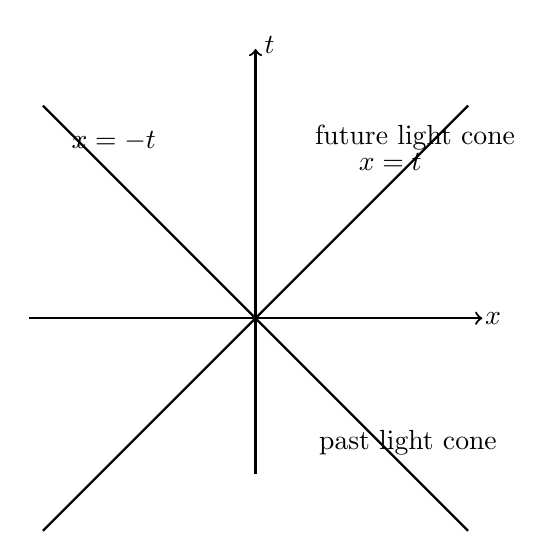
\begin{tikzpicture}[scale=0.9]
\draw[->,thick] (-3.2,0) -- (3.2,0);
\draw[->,thick] (0,-2.2) -- (0,3.8);
\draw (3.35,0) node {$x$};
\draw (0.2,3.85) node {$t$};

\draw[thick] (-3,3) -- (0,0) -- (3,3);
\draw[thick] (-3,-3) -- (0,0) -- (3,-3);

\draw (2.25,2.55) node {future light cone};
\draw (2.15,-1.75) node {past light cone};
\draw (-2.0,2.5) node {$x=-t$};
\draw (1.9,2.2) node {$x=t$};
\end{tikzpicture}
\hspace{1cm}
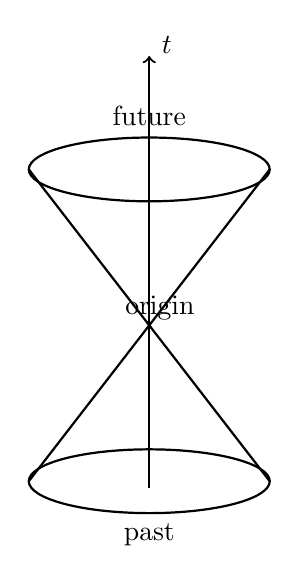
\begin{tikzpicture}[scale=0.9]
\draw[->,thick] (0,-2.3) -- (0,3.8);
\draw (0.25,3.95) node {$t$};

\draw[thick] (0,0) -- (-1.7,2.2);
\draw[thick] (0,0) -- (1.7,2.2);
\draw[thick] (0,0) -- (-1.7,-2.2);
\draw[thick] (0,0) -- (1.7,-2.2);

\draw[thick] (0,2.2) ellipse (1.7 and 0.45);
\draw[thick] (0,-2.2) ellipse (1.7 and 0.45);

\draw (0,2.95) node {future};
\draw (0,-2.95) node {past};
\draw (0.15,0.25) node {origin};
\end{tikzpicture}
\caption{Two ways of drawing the null structure. On the left is the \(1+1\)-dimensional light cone; on the right is a schematic cone picture for higher-dimensional spacetime.}
\end{figure}

The terminology then becomes natural. The future light cone is the set of events that can be reached by a light signal emitted from the origin. The past light cone is the set of events that can send a light signal to the origin. Nothing deep is hidden in the terminology itself; what matters is the null condition that defines these sets.

\subsection{Question \& Answer}

\paragraph{Question.} If special relativity has the invariant \(\tau^2=t^2-x^2-y^2-z^2\), what is the corresponding invariant in Newtonian mechanics?

\paragraph{Answer.} Simply the time interval. Newtonian mechanics assumes that all inertial observers agree on \(\Delta t\). Relativity gives up that universal time and replaces it by an invariant spacetime interval.

\section{From Ordinary Vectors to Four-Vectors}

With the invariant interval in hand, the lecture introduces notation. The move is deliberate: only after the geometry is clear do we compress the symbols.

The simplest ordinary vector in three-dimensional space is the displacement between two points. If we place its tail at the origin, the vector is specified by the three numbers
\begin{equation}
x^i=(x,y,z),
\qquad i=1,2,3.
\end{equation}
Now suppose we want not only the position of an event but also the time at which it occurs. Then the natural object is four-dimensional:
\begin{equation}
x^\mu=(t,x,y,z),
\qquad \mu=0,1,2,3.
\end{equation}
The historical convention adopted in the lecture is that time is the zeroth component,
\begin{equation}
x^0=t,
\qquad
x^1=x,
\qquad
x^2=y,
\qquad
x^3=z.
\end{equation}
With this notation, the interval may be written compactly as
\begin{equation}
\tau^2=(x^0)^2-(x^1)^2-(x^2)^2-(x^3)^2.
\end{equation}

This is mostly organization, but it is organization with a purpose. Just as ordinary vectors transform linearly under rotations of spatial coordinates, four-vectors transform linearly under Lorentz transformations. The lecture makes the point in a practical way: one may regard the Lorentz transformation as a matrix acting on a column vector of components. The physics has not changed. What has changed is the language in which the physics is packaged.

\section{Small Intervals and Four-Velocity}

The final move in the lecture is from finite displacements to small ones. Instead of thinking about the position of an event relative to an origin, we think about a short segment along a worldline. Let
\begin{equation}
\Delta x^\mu=(\Delta t,\Delta x,\Delta y,\Delta z)
\end{equation}
be such a small spacetime interval. The invariant separation associated with it is
\begin{equation}
\Delta\tau^2=\Delta t^2-\Delta x_i\Delta x_i
=\Delta t^2-\Delta x^2-\Delta y^2-\Delta z^2.
\end{equation}

Now compare ordinary velocity with the relativistic construction. In ordinary mechanics, velocity is formed by dividing a spatial displacement by a time interval, and it has only spatial components. Here we divide the four-displacement by the invariant proper-time interval:
\begin{equation}
u^\mu=\frac{\Delta x^\mu}{\Delta\tau}.
\end{equation}
This is the four-velocity. It has four components, not three. In a continuum notation, the same definition becomes
\begin{equation}
u^\mu=\frac{dx^\mu}{d\tau}.
\end{equation}

\begin{figure}[t]
\centering
\begin{tikzpicture}[scale=0.95]
\draw[->,thick] (-0.2,0) -- (4.8,0);
\draw[->,thick] (0,-0.2) -- (0,4.8);
\draw (4.95,0) node {$x$};
\draw (0.2,4.95) node {$t$};

\draw[thick] (0.5,0.5) .. controls (1.2,1.1) and (1.8,2.0) .. (2.5,2.8)
             .. controls (3.0,3.35) and (3.45,3.75) .. (4.1,4.2);

\draw[thick] (2.38,2.66) -- (2.92,3.18);
\draw (3.45,3.25) node {$\Delta x^\mu$};
\draw (2.05,2.15) node {$\Delta\tau$};
\end{tikzpicture}
\caption{A short segment along a worldline. The lecture first treats this as a small discrete interval and only later lets it become differential.}
\end{figure}

The lecture stops at precisely the right place. We are not yet given the full relativistic dynamics of particles, but we are told where we are going. Position, velocity, acceleration, momentum, and energy will all be reorganized in terms of four-vectors. This chapter ends at the threshold of that program.

\section{Summary}

The lecture begins by rebuilding the railroad-track picture and reminding us that the speed of light is set to \(1\) by choice of units. It then shows how to read the motion of a frame directly from the Lorentz transformation by setting its spatial origin equal to zero. Repeating that trick for a third observer produces the velocity-addition law
\[
w=\frac{u+v}{1+uv},
\]
or, in conventional units,
\[
w=\frac{u+v}{1+\dfrac{uv}{c^2}}.
\]

From there the argument broadens. The invariant interval
\[
\tau^2=t^2-x^2-y^2-z^2
\]
becomes the central object; light rays are characterized by the null condition \(\tau^2=0\); and the language of four-vectors condenses the geometry into a form ready for dynamics. The final definition,
\[
u^\mu=\frac{\Delta x^\mu}{\Delta\tau},
\]
is therefore not a side remark. It is the beginning of relativistic mechanics.